%==============================================================================
%  PART 2 --- THE INGESTION PIPELINE (Task 1)
%  Chapters: Architecture & Storage | Data Ingestion | Linking | NLP Enrichment
%==============================================================================

\chapter{System Architecture and Storage}
\label{ch:architecture}

This chapter describes the architecture of the ingestion pipeline (Task~1) and
motivates the storage solution, which the assignment singles out as a graded design
choice.

\section{Architecture overview}
PolySignal is a sequence of loosely coupled modules, each with a typed input
contract, a typed output contract, and no knowledge of how its neighbours are
implemented. Data flows in one direction --- from external sources to the dashboard
--- and is persisted at every stage, so any stage can be re-run, audited, or replaced
in isolation. \Cref{fig:arch} shows the flow.

\begin{figure}[H]
\centering
\resizebox{\linewidth}{!}{%
\begin{tikzpicture}[
  font=\sffamily\small,
  node distance=6mm and 9mm,
  src/.style={draw=psgrey,fill=pslightgrey,rounded corners=2pt,minimum height=8mm,inner xsep=5pt,align=center},
  stage/.style={draw=psblue,fill=psblue!10,rounded corners=3pt,minimum height=11mm,minimum width=20mm,align=center,thick},
  store/.style={draw=psorange,fill=psorange!12,rounded corners=3pt,minimum height=11mm,align=center,thick},
  result/.style={draw=psgreen,fill=psgreen!12,rounded corners=3pt,minimum height=11mm,align=center,thick},
  arr/.style={-{Stealth[length=2mm]},psgrey,thick}
]
% sources
\node[src] (poly) {Polymarket\\Gamma\,/\,CLOB};
\node[src,below=3mm of poly] (tg) {Telegram\\(Telethon)};
\node[src,below=3mm of tg] (rd) {Reddit\\(Scrapling)};
\node[src,below=3mm of rd] (x) {X/Twitter\\(Playwright)};
\node[draw=psgrey,dashed,fit=(poly)(tg)(rd)(x),inner sep=4pt,label=above:{\footnotesize external sources}] (sources) {};

\node[stage,right=10mm of tg] (ing) {Ingestion\\\& normalise};
\node[store,right=of ing] (parq) {Parquet\\data lake};
\node[stage,right=of parq] (link) {Contract--post\\linking};
\node[stage,below=8mm of link] (nlp) {NLP\\enrichment\\\& stance};
\node[store,left=of nlp] (graph) {Neo4j\\knowledge\\graph};
\node[stage,left=of graph] (feat) {Social\\Pressure\\Index};
\node[result,below=8mm of feat] (eval) {Leakage-free\\backtest};
\node[result,right=of eval] (dash) {React\\dashboard};

\draw[arr] (sources.east) -- (ing.west);
\draw[arr] (ing) -- (parq);
\draw[arr] (parq) -- (link);
\draw[arr] (link) -- (nlp);
\draw[arr] (nlp) -- (graph);
\draw[arr] (nlp) to[bend left=8] (feat);
\draw[arr] (graph) -- (feat);
\draw[arr] (feat) -- (eval);
\draw[arr] (eval) -- (dash);
\draw[arr] (parq.south) to[bend right=22] (feat.north);
\end{tikzpicture}}
\caption{End-to-end architecture. Blue nodes are processing stages, orange nodes are
stores, green nodes are user-facing outputs. Parquet is the analytical source of
truth; Neo4j is a queryable projection of it.}
\label{fig:arch}
\end{figure}

\section{Storage solution and its motivation}
\label{sec:storage}
The dataset has three characteristics that drive the storage choice: it is
\emph{strongly temporal} (price series and longitudinal posts), it is
\emph{schema-heterogeneous} across platforms, and it is queried mostly by
\emph{wide columnar scans and aggregations} (group-by domain, by month, by market)
rather than by point look-ups. We adopt a \textbf{two-store design}.

\paragraph{Apache Parquet as the analytical source of truth.}
All normalised and analytical tables are stored as Apache Parquet
files~\cite{apachearrow}. Parquet is a good fit for this workload for several
concrete reasons:
\begin{itemize}
  \item \textbf{Columnar layout.} Analyses read a few columns over millions of rows
  (e.g.\ \code{price} over time, \code{sentiment\_compound} by platform); a columnar
  format reads only those columns and skips the rest, with per-column compression
  that shrinks the ${\sim}1.37$M-post corpus from gigabytes of JSON to a few hundred
  megabytes.
  \item \textbf{Schema-on-write with evolution.} A single \code{SocialPostRecord}
  schema absorbs Reddit and Telegram, whose native shapes differ; new optional
  columns (the enrichment fields) are added as \emph{derived tables} keyed by
  \code{post\_id} rather than by rewriting the corpus, preserving the raw data.
  \item \textbf{Engine portability.} The same files are read by pandas/PyArrow on a
  laptop and by Apache Spark~\cite{zaharia2016spark} at scale, with no migration. The
  ``data zones'' below are laid out so that a Hive-style partitioned write
  (\code{platform=}/\code{domain=}/\code{date=}) is an additive change.
\end{itemize}

\noindent The data lake is partitioned by \emph{maturity} into zones, summarised in
\Cref{tab:zones}. This separation keeps immutable provenance (\code{raw/}) apart from
validated records (\code{normalized/}) and from analysis-ready features
(\code{analytical/}), which is what makes the pipeline auditable and re-runnable.

\begin{table}[H]
\centering
\caption{Data zones, partitioned by maturity.}
\label{tab:zones}
\small
\begin{tabularx}{\linewidth}{@{}l X l@{}}
\toprule
\textbf{Zone} & \textbf{Purpose} & \textbf{Format}\\
\midrule
\code{raw/}        & API payloads and social snapshots with retrieval lineage & JSON / JSONL\\
\code{normalized/} & validated, typed, deduplicated records & Parquet\\
\code{analytical/} & feature tables, evidence, timelines, backtests & Parquet / JSON\\
\code{cache/}      & LLM responses and expensive intermediates, keyed deterministically & JSON / Parquet\\
\code{graph\_exports/} & offline graph dumps for backup & CSV / JSONL\\
\bottomrule
\end{tabularx}
\end{table}

\paragraph{Neo4j as a relationship projection.}
Questions such as ``which authors bridge the crypto and macro discussions?'' or
``what is the stance neighbourhood of this contract?'' are graph traversals, awkward
to express as columnar joins. We therefore project the Parquet tables into a
\textbf{Neo4j} property graph~\cite{robinson2015graph}, which is canonical for
relationship analysis but \emph{not} a replacement for time-series storage --- price
points deliberately stay in Parquet. The schema is detailed in \Cref{sec:graph}.

\begin{takeaway}
\textbf{Design choice.} Parquet for analytical, columnar, temporal scans;
Neo4j for relationship traversal. Each store is used only for what it is best at, and
Parquet remains the single source of truth.
\end{takeaway}

\section{Knowledge-graph schema}
\label{sec:graph}
The Neo4j projection models the domain as a property graph
(\Cref{tab:graph}). Contracts, outcomes, posts, authors, platforms, and domains are
nodes; linking and stance become typed, evidence-bearing relationships. A
\code{:LINKED\_TO} edge is created only for \emph{accepted} evidence (the policy of
\Cref{ch:linking}). Directional stance is modelled with a \emph{single}
\code{:SUPPORTS} edge that points from a post to the specific \code{:Outcome} node it
argues for: a post backing \textsc{No} becomes a \code{:SUPPORTS} edge to that
contract's \textsc{No} outcome, so the edge's \emph{target} already encodes the
direction and a separate \code{:OPPOSES} type is unnecessary. Only
\code{supports\_yes}/\code{supports\_no} stances are projected; neutral, ambiguous, and
insufficient-context rows are reported as skipped rather than projected. Price points
stay in Parquet, since time-series
analysis does not benefit from millions of graph nodes. Loading is idempotent
(batched \code{MERGE} on \code{UNWIND} payloads), so the graph can be rebuilt from
the Parquet tables at any time.

\begin{table}[H]
\centering
\caption{Knowledge-graph contents derived from the current pipeline artifacts (the
loader is idempotent over the Parquet tables, so each edge count equals its artifact
count). Directional stance is a single \code{:SUPPORTS} edge to the supported outcome
node, which removes the need for a redundant, always-empty \code{:OPPOSES} type.}
\label{tab:graph}
\small
\begin{tabular}{@{}l r @{\hskip 2.4em} l r@{}}
\toprule
\textbf{Relationship} & \textbf{Count} & \textbf{Relationship} & \textbf{Count}\\
\midrule
\code{:BELONGS\_TO} (contract$\to$domain) & 300 & \code{:LINKED\_TO} (post$\to$contract) & 37{,}562\\
\code{:HAS\_OUTCOME}                       & 600 & \code{:SUPPORTS} (post$\to$outcome)    & 6{,}569\\
\code{:POSTED\_ON} (post$\to$platform)    & 1{,}368{,}041 & \code{:WROTE} (author$\to$post) & 1{,}367{,}960\\
\bottomrule
\end{tabular}
\end{table}


%==============================================================================
\chapter{Data Ingestion}
\label{ch:ingestion}

\section{Polymarket contracts and price series}
Contracts are collected from Polymarket's public \textbf{Gamma} API (market metadata)
and \textbf{CLOB} API (price history)~\cite{polymarketdocs}. A binary filter keeps only
\textsc{Yes}/\textsc{No} contracts; multi-outcome and team-vs-team markets are detected,
logged with a reason, and skipped. The normaliser maps Polymarket identifiers to our
schema (\code{conditionId}$\rightarrow$\code{market\_id}, per-outcome CLOB token ids
$\rightarrow$\code{outcome\_id}) and writes the three contract tables of
\Cref{tab:schema-market}.

\paragraph{Full-lifetime price reconstruction.}
A practical obstacle is that the CLOB \code{/prices-history} endpoint returns only a
narrow window for a settled market and rejects ranges longer than ${\sim}$two weeks.
To obtain a \emph{complete} probability trajectory --- which Task~2 requires --- the
ingester walks each contract's lifetime in 14-day windows and merges them, upserting
on \code{(market\_id, outcome\_id, timestamp)} so repeated fetches never duplicate
samples. Contracts for which a continuous timeline cannot be reconstructed are
reported and excluded.

\section{Social-media collection}
\label{sec:social-collection}
Social posts are collected longitudinally so that, for each contract, discussion
spanning creation-to-resolution is available.

\paragraph{Telegram (primary).} Public channels and groups are read through the
official MTProto API using Telethon~\cite{telethon}. Collection pages backwards
through each channel's history by message id, checkpointing after every batch so a
killed run resumes exactly where it stopped; Telegram's rate limits
(\code{FloodWait}) are honoured automatically. Telegram supplies the overwhelming
majority of the corpus (\Cref{tab:corpus}).

\paragraph{Reddit (secondary).} Reddit is collected via compliant public-web scraping
with Scrapling~\cite{scrapling} against \code{old.reddit.com}; the official OAuth API
is not used. When Reddit returns \code{HTTP 403/429}, the collector opens a circuit
breaker and respects a cooldown --- it reports the block rather than evading it ---
so Reddit coverage is built up opportunistically over repeated, rate-limited passes.

\paragraph{X/Twitter (third platform, small but real).} X is collected through
\textbf{authenticated browser automation} (Playwright~\cite{playwright}): a logged-in
session driven from market-derived search queries, with the same checkpointing and
rate-limiting discipline as the other collectors. X's anti-automation defences (token
challenges, login walls, and aggressive \code{HTTP 429} rate limiting) cap how much can
be gathered responsibly, so X is a \textbf{small third platform --- 2{,}822 posts}
(\Cref{tab:corpus}) --- rather than a major contributor. It is nonetheless genuinely
present: X posts flow through the same platform-agnostic schema and enter the
cross-platform analysis (\Cref{ch:crossplatform}), where 114 contracts carry all three
sources.

\paragraph{Comments and replies.} For a sample of high-evidence posts the collector
also retrieves a bounded sample of \emph{replies/comments} --- their text, author,
timestamp, and per-comment engagement --- satisfying the \code{comments} field of the
schema.

\paragraph{Why no synthetic padding.} Where a source is sparse, the corpus stays
sparse. We never synthesise posts to inflate coverage; the consequences of this
honesty are analysed in \Cref{ch:limitations} rather than hidden.

\begin{table}[H]
\centering
\caption[Composition of the social corpus]{Composition of the analysed social corpus
(deduplicated). All three platforms are present; Telegram dominates, while X/Twitter is
a small third platform whose scale is capped by its anti-automation defences
(\Cref{sec:scope}).}
\label{tab:corpus}
\small
\begin{tabular}{@{}l r r@{}}
\toprule
\textbf{Platform} & \textbf{Posts} & \textbf{Share}\\
\midrule
Telegram   & 1{,}348{,}965 & 98.6\%\\
Reddit     & 16{,}254      & 1.2\%\\
X/Twitter  & 2{,}822       & 0.2\%\\
\midrule
\textbf{Total} & \textbf{1{,}368{,}041} & 100\%\\
\bottomrule
\end{tabular}
\end{table}

\section{Market-aware query generation}
\label{sec:querygen}
Reddit retrieval and the targeted Telegram searches are driven by queries generated
\emph{from each contract question}. A naive keyword extractor would discard the
load-bearing constraint in a question such as ``Will China invade Taiwan
\emph{before GTA VI}?''. The generator instead decomposes a question into an
\emph{event core}, its \emph{constraints}, and \emph{context anchors}, and emits a
small, deduplicated family of query types --- \emph{core}, \emph{entity},
\emph{constraint}, \emph{anchor} (including Roman$\leftrightarrow$Arabic numeral
variants), \emph{slug}, \emph{domain}, \emph{tag}, and \emph{polymarket}. Each query
carries trace metadata (\code{market\_id}, \code{query\_type}, \code{rank}) so that
retrieval provenance is preserved on disk and can later inform --- but never by
itself decide --- relevance.

\begin{table}[H]
\centering
\caption[Worked query-generation example]{Query family generated for the contract
\emph{``Will China invade Taiwan before GTA VI?''}. The generator preserves the
load-bearing \emph{constraint} (the \code{before}-anchor) that a naive keyword extractor
would discard, and emits numeral variants so that ``GTA 6'' and ``GTA VI'' both match.}
\label{tab:querygen}
\small
\begin{tabularx}{\linewidth}{@{}l X@{}}
\toprule
\textbf{Query type} & \textbf{Generated query}\\
\midrule
core       & \code{china invade taiwan}\\
entity     & \code{China}, \code{Taiwan}\\
constraint & \code{china taiwan before gta vi}\\
anchor     & \code{GTA VI}, \code{GTA 6} (Roman\,$\leftrightarrow$\,Arabic variant)\\
slug       & \code{will-china-invade-taiwan-before-gta-vi}\\
domain     & \code{geopolitics}, \code{china taiwan war}\\
\bottomrule
\end{tabularx}
\end{table}

\section{Normalisation, timestamps, and deduplication}
Every ingested record is validated against a Pydantic model, its timestamp is
normalised to timezone-aware UTC, and it is deduplicated. The pipeline preserves one
row per \code{(post, query, candidate market, retrieval window)} tuple and flags
later occurrences of the same \code{(platform, post\_id)} as duplicates, so that a
post surfaced by several queries is neither double-counted nor lost as additional
retrieval evidence. After this step the corpus contains no duplicate posts.


%==============================================================================
\chapter{Contract--Post Linking}
\label{ch:linking}

A retrieval query that mentions ``Iran'' returns many posts that have nothing to do
with a \emph{specific} contract about Iran. Linking is the step that decides,
semantically, which posts are genuinely about which contract --- and it is graded by
the assignment as a key design choice.

\section{A deterministic relevance scorer}
The default linker is fully deterministic: no language model is required to reproduce
any number in this report. For each candidate \code{(contract, post)} pair it computes
a relevance score from interpretable signals:
\begin{itemize}
  \item \textbf{entity and term overlap} between the contract question (and its
  slug/description) and the post text, weighted by salience;
  \item \textbf{constraint matching} --- the temporal or contextual constraint of the
  question (a date, a threshold, an anchor event) must be compatible with the post,
  so that a post about ``Bitcoin at \$80k'' is not linked to a ``\$150k'' contract;
  \item \textbf{domain consistency}, penalising cross-domain false matches; and
  \item \textbf{temporal admissibility} --- a post published after the contract closed
  can never be accepted as evidence.
\end{itemize}
Each pair receives a relevance label in \{\code{relevant}, \code{weakly\_relevant},
\code{ambiguous}\} and a calibrated \code{confidence} in $[0,1]$. Concretely, the base
score is a weighted blend of four lexical-semantic overlaps,
\begin{equation}
\text{score} = 0.25\,J + 0.35\,T + 0.20\,E + 0.20\,Q \;+\; (\text{gated bonuses})
\;-\; (\text{penalties}),
\label{eq:relevance}
\end{equation}
where $J$ is the Jaccard overlap of token sets, $T$ the salience-weighted term overlap,
$E$ the named-entity overlap, and $Q$ the overlap with the generating query; constraint
matches add gated bonuses, while domain mismatch and temporal inadmissibility apply
penalties. Labels follow fixed cut-offs on the resulting confidence (weakly-relevant at
$\geq\!0.60$, relevant higher), and an optional, cached LLM verifier can be enabled for
borderline rows --- but it was \emph{not} used for the results reported here:
\textbf{all 4{,}112{,}547 candidate pairs were scored by the deterministic baseline}.

\section{From candidates to accepted evidence}
Scoring a pair is not the same as accepting it. The \emph{acceptance policy} ---
applied identically by the graph loader and the evidence exporter --- admits a pair as
real evidence only if it is \code{relevant}, or \code{weakly\_relevant} with
\code{confidence}~$\geq 0.60$; \emph{and} it resolves to an existing parent post and
contract; \emph{and} it is temporally admissible (pre-close, timestamp present);
\emph{and} it survives deduplication (per \code{(contract, post)} only the
highest-confidence row is kept). \Cref{fig:funnel} shows the resulting funnel from the
raw corpus down to accepted evidence.

\begin{figure}[H]
\centering
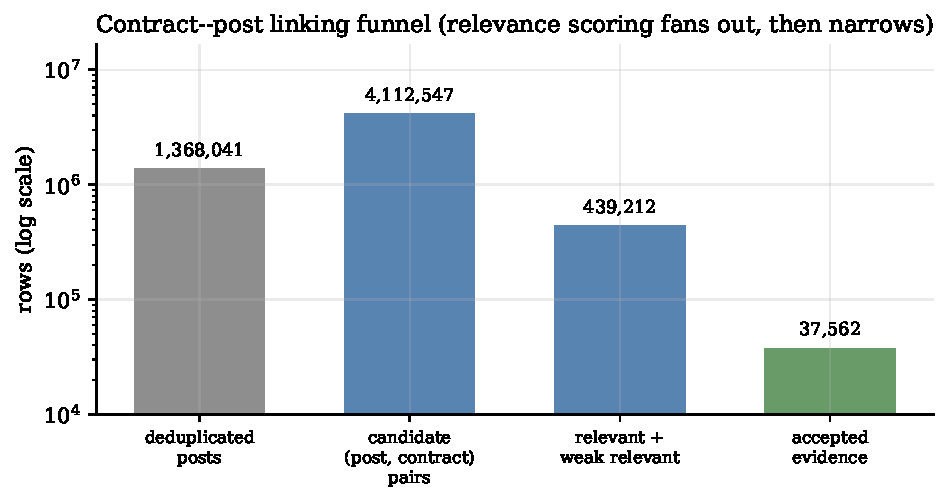
\includegraphics[width=0.92\linewidth]{fig_linking_funnel.pdf}
\caption{The linking funnel (log scale). Relevance scoring fans the corpus out into
\textbf{4{,}112{,}547} candidate (post, contract) pairs, of which only
\textbf{37{,}562} survive the acceptance policy as evidence. The largest losses are the
unrelated majority and the weak links below the confidence floor.}
\label{fig:funnel}
\end{figure}

\Cref{fig:confidence} explains why the funnel narrows so sharply: the bulk of scored
pairs sit in the $0.40$--$0.50$ confidence band, well below the $0.60$ acceptance
threshold. This conservative floor trades recall for precision --- a deliberate choice,
since downstream the cost of a spurious link (a post wrongly attributed to a contract)
is higher than the cost of a missed one.

\begin{figure}[H]
\centering
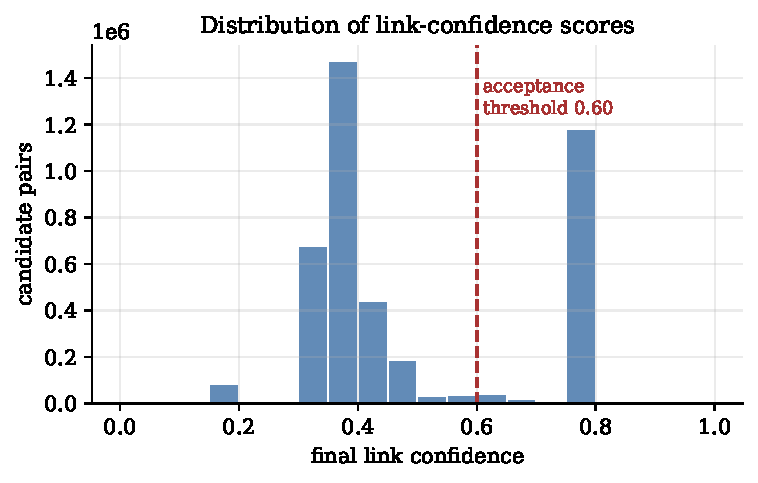
\includegraphics[width=0.74\linewidth]{fig_link_confidence.pdf}
\caption{Distribution of final link-confidence scores over all 4{,}112{,}547 candidates.
The dashed line marks the $0.60$ acceptance threshold for weakly-relevant links; most
candidates fall below it.}
\label{fig:confidence}
\end{figure}

\section{Coverage statistics}
The assignment asks for coverage statistics --- the fraction of contracts with at
least $k$ associated posts. \Cref{tab:link-labels} reports the relevance-label
breakdown, and \Cref{fig:coverage} the depth of accepted evidence per contract.
Accepted evidence reaches \textbf{147 of 300 contracts (49\%)}; 35~contracts have at
least 100 accepted links, while 153~have none. This uneven coverage is the central
data-quality story of the project and is dissected in
\Cref{ch:crossplatform,ch:limitations}.

\begin{table}[H]
\centering
\caption{Relevance labels over all 4{,}112{,}547 scored candidate pairs. Broad
retrieval makes \emph{unrelated} the majority label; the acceptance policy then keeps a
small, high-precision evidence set.}
\label{tab:link-labels}
\small
\begin{tabular}{@{}l r r@{}}
\toprule
\textbf{Relevance label} & \textbf{Pairs} & \textbf{Share}\\
\midrule
relevant         & 26{,}337      & 0.6\%\\
weakly\_relevant & 412{,}875     & 10.0\%\\
ambiguous        & 150{,}352     & 3.7\%\\
unrelated        & 3{,}522{,}983 & 85.7\%\\
\midrule
\textbf{Total scored} & \textbf{4{,}112{,}547} & 100\%\\
\addlinespace[2pt]
\textbf{Accepted as evidence} & \textbf{37{,}562} & 0.9\%\\
\bottomrule
\end{tabular}
\end{table}

\begin{figure}[H]
\centering
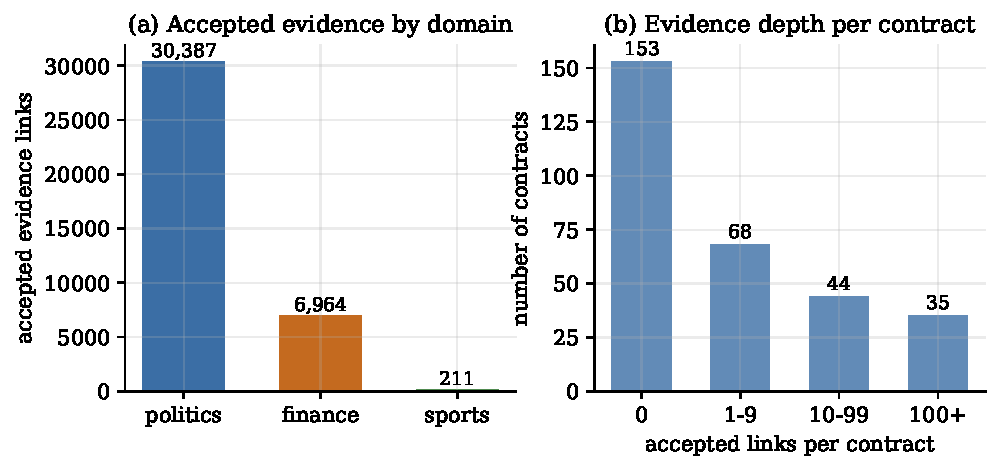
\includegraphics[width=\linewidth]{fig_evidence_coverage.pdf}
\caption{Evidence coverage. (a)~Accepted evidence is dominated by the politics domain
($30{,}387$ links) and almost absent for sports ($211$). (b)~Depth of accepted
evidence per contract: 153 contracts have no accepted evidence, 35 have $\geq 100$
links.}
\label{fig:coverage}
\end{figure}


%==============================================================================
\chapter{Text Preprocessing and NLP Enrichment}
\label{ch:nlp}

Enrichment turns raw post text into the structured fields required by the assignment
(hashtags, mentioned entities, language) and the analytical signals used later
(sentiment, topics, stance). To respect the data-safety convention of never rewriting
the ${\sim}300$\,MB raw corpus, all enrichment is written to \emph{derived tables}
keyed by \code{post\_id}, exactly like the linking and stance outputs. Every backend
degrades gracefully so the pipeline always runs offline, and the chosen backend is
recorded per row.

\section{Normalisation, language, hashtags, entities}
Text is lower-cased and stripped of control characters for matching while the original
is retained for display; timestamps are normalised to UTC (\Cref{ch:ingestion}).
\textbf{Language} is detected with \code{langdetect} when available, otherwise a
Cyrillic/stop-word heuristic; English dominates (1{,}118{,}413 enriched posts), followed
by Russian (105{,}395), reflecting the geopolitics channels. \textbf{Hashtags and
mentions} are extracted by deterministic regular expressions. \textbf{Named entities}
are extracted with spaCy~\cite{honnibal2017spacy} when installed, otherwise a
heuristic gazetteer-plus-capitalised-$n$-gram backend; the run reported here used the
heuristic backend over all \textbf{1{,}368{,}041} enriched posts. Its limitations
(channel handles and news boilerplate leaking in as pseudo-entities) are discussed in
\Cref{ch:discourse}.

\section{Sentiment analysis}
Sentiment is computed with \textbf{VADER}~\cite{hutto2014vader}, a rule-based model
tuned for social text (emoji, capitalisation, slang) and a sensible default that needs
no training data. Each post receives positive/neutral/negative proportions and a
\code{compound} score in $[-1,1]$, thresholded at $\pm 0.05$ into a label. A
transformer backend (\code{twitter-roberta}) is available as an opt-in upgrade. The
distribution of sentiment is analysed in \Cref{ch:discourse}; here we note only that
sentiment is a \emph{generic} polarity signal, deliberately distinct from stance.

\section{Topic modelling}
Topics are extracted with \textbf{Latent Dirichlet Allocation}~\cite{blei2003lda}
over \code{CountVectorizer} features (scikit-learn~\cite{pedregosa2011scikit}), run
over the \emph{linked} posts --- the discourse that actually concerns the contracts.
The vectoriser keeps the top \textbf{2{,}000} alphabetic terms (token pattern
\code{[a-zA-Z]\{2,\}}, unigrams), drops terms appearing in more than $60\%$ of documents
or in fewer than three, and removes both the standard English stop-word list and a
curated set of social/market boilerplate (e.g.\ ``http'', ``rt'', ``amp'', ticker
chatter). LDA is then fit with \textbf{ten topics}, the \code{"batch"} learning method,
\textbf{20} iterations, and a fixed \code{random\_state=42}; each topic is summarised by
its twelve highest-weight terms. We report ten topics as a deliberate, interpretable
granularity rather than tuning topic count by a coherence criterion --- the topics are
used qualitatively, to characterise \emph{what} the linked discourse is about, not as a
predictive feature. The resulting topics and their interpretation are presented in
\Cref{ch:discourse}.

\section{Outcome-aware stance}
\label{sec:stance}
Stance is the directional signal that feeds prediction, and it is computed
\emph{relative to each contract's outcomes}, not as generic polarity. For every
accepted \code{(contract, post)} link the stance module interprets the post against the
\textsc{Yes}/\textsc{No} proposition using outcome-specific cues, negation handling,
and uncertainty markers, emitting a label in \{\code{supports\_yes},
\code{supports\_no}, \code{neutral}, \code{ambiguous}, \code{insufficient\_context}\}
with a confidence. The deterministic heuristic labelled \textbf{35{,}679} post--outcome
rows across 140 contracts; \Cref{fig:stance} shows the distribution.

\begin{figure}[H]
\centering
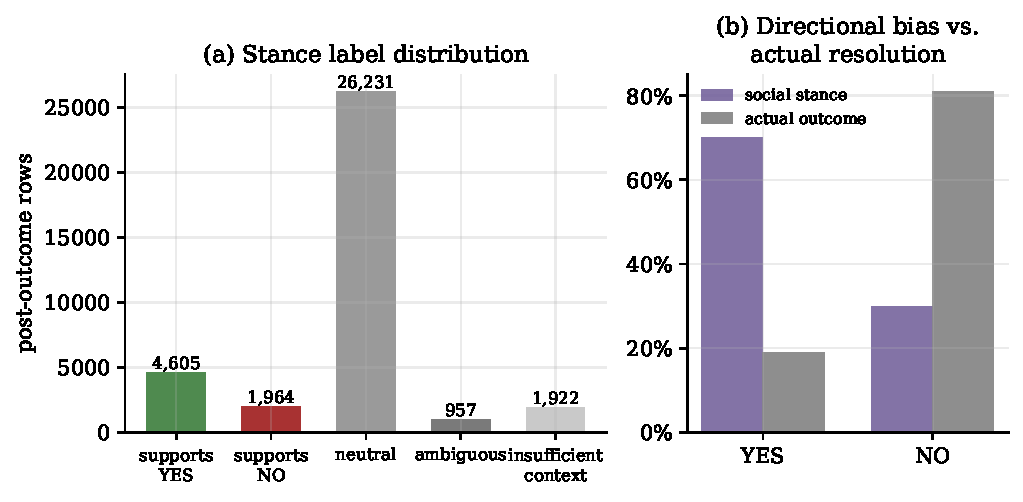
\includegraphics[width=\linewidth]{fig_stance.pdf}
\caption{Outcome-aware stance. (a)~Most rows are \code{neutral} (26{,}231); directional
rows split 4{,}605 \textsc{Yes} vs.\ 1{,}964 \textsc{No}. (b)~The social stance is
\textbf{2.3:1 biased towards \textsc{Yes}}, whereas the contracts actually resolve
\textbf{4.3:1 towards \textsc{No}} --- the optimism/hype mismatch that recurs
throughout the predictive analysis.}
\label{fig:stance}
\end{figure}

\begin{takeaway}
\textbf{Sentiment vs.\ stance.} Sentiment (VADER) measures the mood of the text;
stance measures its directional position on a contract's outcome. Both are computed,
but only stance feeds the forecast --- and stance already reveals a systematic
\textsc{Yes}-bias that foreshadows the predictive null result.
\end{takeaway}
